\section{Inferring the weight sharing scheme}
\label{sec:trans}

\subsection{Methodology}

As we saw in \secref{sec:sym} (\figref{fig:rect}), the classical convolution on grid graphs can be obtained visually by translating a rectangular window over the pixel domain. The idea of this section is to define similarly a convolution on graph domains, using a notion of translation defined on graphs~\citep{pasdeloup2017translations}. The translations we use match Euclidean translations on 2D grid graphs~\citep{GrePasViaGri201610}, and extend them on general ones, by preserving three simple key properties: injectivity, edge-constraint, and neighborhood-preservation, which we will detail later.

Given a set of graph translations $\ct = \{t_i, i \in \seq{\kappa - 1}\} \cup \{t_0 = \id \}$, the corresponding convolution can be expressed using the same formalism we used in \chapref{chap:2}, as:
\begin{gather}
w \ast x = \displaystyle\sum_{t \in \ct} w[t] \h{2} t(x)
\end{gather}
where $x$ is a signal over vertices of a graph $\gve$, and $w$ is a signal defined on $\ct \subset \Phi_{\EC}(G)$. Depending on the algebraic nature of $\ct$ (that we will discuss later), the theoretical results obtained in \chapref{chap:2} hold. Under the ternary representation, finding such translations amounts to infer the weight sharing scheme $S$.

By denoting $w_i = w[t_i]$, we obtain the more familiar expression:
\begin{gather}
\forall u \in V, w \ast x [u] = \displaystyle\sum_{i=0}^{\kappa-1} w_i \h{2} x[t_i^{-1}(u)]
\end{gather}
This expression extends the definition of convolutions from grid graphs to general graphs, with the use of graph translations. We use it to obtain extended CNNs that can be applied on graphs. In this manuscript, we coin the term \emph{Translation-convolutional neural network} (TCNN) to refer to them, but they are the same as the extended convolutions we defined in \cite{pasdeloup2017convolutional}.

Besides defining translation-convolution on general graphs, designing a TCNN also implies extending the other building blocks of classical CNNs. As a counterpart for pooling operations, we define a graph subsampling and apply strided translation-convolution. The translations of the subsampled graph are derived from those of the base graph to define translation-convolution at the downscaled level. We will also use a weak form of data augmentation using these translations. \figref{fig:outline} depicts the proposed methodology~\citep{lassance2018matching}.

\begin{figure}[h!p]
\begin{framed}
  Step 0 (optional): infer a graph (see \cite{pasdeloup2017convolutional})
  \begin{center}
    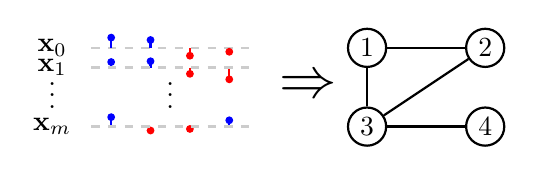
\begin{tikzpicture}[thick]
      \node at (0,0) {$\mathbf{x}_0$};
      \path[black!20!white, dashed]
      (0.5,0) edge (2.5,0);
      \path
      (0.75, 0) edge[blue] (0.75, 0.13)
      (1.25, 0) edge[blue] (1.25, 0.1)
      (1.75, 0) edge[red] (1.75, -0.1)
      (2.25, 0) edge[red] (2.25, -0.05);
      \node[fill, circle, inner sep = 1pt, blue] at (0.75, 0.13) {};
      \node[fill, circle, inner sep = 1pt, blue] at (1.25, 0.1) {};
      \node[fill, circle, inner sep = 1pt, red] at (1.75, -0.1) {};
      \node[fill, circle, inner sep = 1pt, red] at (2.25, -0.05) {};
      \node at (0,-0.25) {$\mathbf{x}_1$};
      \begin{scope}[yshift=-0.25cm]
        \path
        (0.75, 0) edge[blue] (0.75, 0.07)
        (1.25, 0) edge[blue] (1.25, 0.08)
        (1.75, 0) edge[red] (1.75, -0.08)
        (2.25, 0) edge[red] (2.25, -0.15);
        \node[fill, circle, inner sep = 1pt,blue] at (0.75, 0.07){};
        \node[fill, circle, inner sep = 1pt,blue] at (1.25, 0.08){};
        \node[fill, circle, inner sep = 1pt,red] at (1.75, -0.08){};
        \node[fill, circle, inner sep = 1pt,red] at (2.25, -0.15){};        
      \end{scope}

      \path[black!20!white, dashed]
      (0.5,-0.25) edge (2.5,-0.25);
      \node at (0,-0.5) {\vdots};
      \node at (0,-1) {$\mathbf{x}_m$};
      \begin{scope}[yshift=-1cm]
        \path
        (0.75, 0) edge[blue] (0.75, 0.12)
        (1.25, 0) edge[red] (1.25, -0.05)
        (1.75, 0) edge[red] (1.75, -0.03)
        (2.25, 0) edge[blue] (2.25, 0.08);
        \node[fill, circle, inner sep = 1pt, blue] at (0.75, 0.12){};
        \node[fill, circle, inner sep = 1pt, red] at (1.25, -0.05){};
        \node[fill, circle, inner sep = 1pt, red] at (1.75, -0.03){};
        \node[fill, circle, inner sep = 1pt, blue] at (2.25, 0.08){};        
      \end{scope}
      \node at (1.5,-0.5) {\vdots};
      \path[black!20!white, dashed]
      (0.5,-1) edge (2.5,-1);

      \node at (3.25, -0.5) {\huge{$\Rightarrow$}};

      \begin{scope}[xshift=4cm]
        \node[draw, circle](a) at (0,0) {1};
        \node[draw, circle](b) at (1.5,0) {2};
        \node[draw, circle](c) at (1.5,-1) {4};
        \node[draw, circle](d) at (0,-1) {3};
      \end{scope}
      \path
      (a) edge (b)
      edge (d)
      (b) edge (d)
      (c) edge (d);
    \end{tikzpicture}
  \end{center}
  
  Step 1: infer translations
  \begin{center}
    \begin{tikzpicture}[thick]      
      \begin{scope}[xshift=0cm]
        \node[draw, circle](a) at (0,0) {1};
        \node[draw, circle](b) at (1.5,0) {2};
        \node[draw, circle](c) at (1.5,-1) {4};
        \node[draw, circle](d) at (0,-1) {3};
      \end{scope}
      \path
      (a) edge (b)
      edge (d)
      (b) edge (d)
      (c) edge (d);
      \node at (2.75, -0.5) {\huge{$\Rightarrow$}};
      \begin{scope}[xshift=4cm, scale=0.5, yshift=0.5cm]
        \node[draw, inner sep=2pt, circle](a) at (0,0) {};
        \node[draw, inner sep=2pt, circle](b) at (1.5,0) {};
        \node[draw, inner sep=2pt, circle](c) at (1.5,-1) {};
        \node[draw, inner sep=2pt, circle](d) at (0,-1) {};
      \end{scope}
      \path[black!20!white]
      (a) edge (b)
      edge (d)
      (b) edge (d)
      (c) edge (d);
      \path[->,>=stealth']
      (a) edge (b)      
      (d) edge (c);
      \begin{scope}[xshift=4cm, scale=0.5, yshift=-1.5cm]
        \node[draw, inner sep=2pt, circle](a) at (0,0) {};
        \node[draw, inner sep=2pt, circle](b) at (1.5,0) {};
        \node[draw, inner sep=2pt, circle](c) at (1.5,-1) {};
        \node[draw, inner sep=2pt, circle](d) at (0,-1) {};
      \end{scope}
      \path[black!20!white]
      (a) edge (b)
      edge (d)
      (b) edge (d)
      (c) edge (d);
      \path[->,>=stealth']
      (b) edge (a)      
      (c) edge (d);
      \begin{scope}[xshift=5.5cm, scale=0.5, yshift=0.5cm]
        \node[draw, inner sep=2pt, circle](a) at (0,0) {};
        \node[draw, inner sep=2pt, circle](b) at (1.5,0) {};
        \node[draw, inner sep=2pt, circle](c) at (1.5,-1) {};
        \node[draw, inner sep=2pt, circle](d) at (0,-1) {};
      \end{scope}
      \path[black!20!white]
      (a) edge (b)
      edge (d)
      (b) edge (d)
      (c) edge (d);
      \path[->,>=stealth']
      (a) edge (d);
      \begin{scope}[xshift=5.5cm, scale=0.5, yshift=-1.5cm]
        \node[draw, inner sep=2pt, circle](a) at (0,0) {};
        \node[draw, inner sep=2pt, circle](b) at (1.5,0) {};
        \node[draw, inner sep=2pt, circle](c) at (1.5,-1) {};
        \node[draw, inner sep=2pt, circle](d) at (0,-1) {};
      \end{scope}
      \path[black!20!white]
      (a) edge (b)
      edge (d)
      (b) edge (d)
      (c) edge (d);
      \path[->,>=stealth']
      (d) edge (a);
    \end{tikzpicture}
  
  \end{center}
  
  Step 2: design convolution weight-sharing

  \begin{center}
    \begin{tikzpicture}[thick]      
      \begin{scope}[xshift=0cm, scale=0.75, yshift=0.5cm]
        \node[inner sep=2pt](w) at (-1.0,-0.5) {$w_1 \times$};
        \node[draw, inner sep=2pt, circle](a) at (0,0) {};
        \node[draw, inner sep=2pt, circle](b) at (1.5,0) {};
        \node[draw, inner sep=2pt, circle](c) at (1.5,-1) {};
        \node[draw, inner sep=2pt, circle](d) at (0,-1) {};       
      \end{scope}
      \path[black!20!white]
      (a) edge (b)
      edge (d)
      (b) edge (d)
      (c) edge (d);
      \path[->,>=stealth']
      (a) edge (b)      
      (d) edge (c);
      \begin{scope}[xshift=0cm, scale=0.75, yshift=-1.5cm]
        \node[inner sep=2pt](w) at (-1.0,-0.5) {+ $w_2 \times$};
        \node[draw, inner sep=2pt, circle](a) at (0,0) {};
        \node[draw, inner sep=2pt, circle](b) at (1.5,0) {};
        \node[draw, inner sep=2pt, circle](c) at (1.5,-1) {};
        \node[draw, inner sep=2pt, circle](d) at (0,-1) {};
      \end{scope}
      \path[black!20!white]
      (a) edge (b)
      edge (d)
      (b) edge (d)
      (c) edge (d);
      \path[->,>=stealth']
      (b) edge (a)      
      (c) edge (d);
      \begin{scope}[xshift=2.5cm, scale=0.75, yshift=0.5cm]
        \node[inner sep=2pt](w) at (-1.0,-0.5) {+ $w_3 \times$};
        \node[draw, inner sep=2pt, circle](a) at (0,0) {};
        \node[draw, inner sep=2pt, circle](b) at (1.5,0) {};
        \node[draw, inner sep=2pt, circle](c) at (1.5,-1) {};
        \node[draw, inner sep=2pt, circle](d) at (0,-1) {};
      \end{scope}
      \path[black!20!white]
      (a) edge (b)
      edge (d)
      (b) edge (d)
      (c) edge (d);
      \path[->,>=stealth']
      (a) edge (d);
      \begin{scope}[xshift=2.5cm, scale=0.75, yshift=-1.5cm]
        \node[inner sep=2pt](w) at (-1.0,-0.5) {+ $w_4 \times$};      
        \node[draw, inner sep=2pt, circle](a) at (0,0) {};
        \node[draw, inner sep=2pt, circle](b) at (1.5,0) {};
        \node[draw, inner sep=2pt, circle](c) at (1.5,-1) {};
        \node[draw, inner sep=2pt, circle](d) at (0,-1) {};
      \end{scope}
      \path[black!20!white]
      (a) edge (b)
      edge (d)
      (b) edge (d)
      (c) edge (d);
      \path[->,>=stealth']
      (d) edge (a);

      \begin{scope}[xshift=5.0cm, scale=0.75, yshift=-0.5cm]
        \node[inner sep=2pt](w) at (-1.0,-0.5) {+ $w_0 \times$};
        \node[draw, inner sep=2pt, circle](a) at (0,0) {};
        \node[draw, inner sep=2pt, circle](b) at (1.5,0) {};
        \node[draw, inner sep=2pt, circle](c) at (1.5,-1) {};
        \node[draw, inner sep=2pt, circle](d) at (0,-1) {};
      \end{scope}
      \path[black!20!white]
      (a) edge (b)
      edge (d)
      (b) edge (d)
      (c) edge (d);
      \path[]
      (a) edge [loop above] (a)
      (b) edge [loop above] (b)
      (c) edge [loop below] (c)
      (d) edge [loop below] (d);

    \end{tikzpicture}
  
  \end{center}
  
  Step 3: design data augmentation
  \begin{center}
    \begin{tikzpicture}[thick]      
      \begin{scope}[xshift=0cm]
        \node[draw, inner sep = 2pt, circle](a) at (0,0) {};
        \node[draw, inner sep = 2pt, circle](b) at (1.5,0) {};
        \node[draw, inner sep = 2pt, circle](c) at (1.5,-1) {};
        \node[draw, inner sep = 2pt, circle](d) at (0,-1) {};
        \path[]
        (0, 0) edge[blue] (0, 0.52)
        (1.5, 0) edge[blue] (1.5, 0.4)
        (0, -1) edge[red] (0, -1.4)
        (1.5, -1) edge[red] (1.5, -1.2);
        \node[fill, circle, inner sep = 1pt, blue] at (0, 0.52) {};
        \node[fill, circle, inner sep = 1pt, blue] at (1.5, 0.4) {};
        \node[fill, circle, inner sep = 1pt, red] at (0, -1.4) {};
        \node[fill, circle, inner sep = 1pt, red] at (1.5, -1.2) {};
      \end{scope}
      \node at (-0.5,-0.5) {$\mathbf{x}_0$};
      \path[black!20!white]
      (a) edge (b)
      edge (d)
      (b) edge (d)
      (c) edge (d);
      \node at (2.25, -0.5) {\huge{$\Rightarrow$}};
      \begin{scope}[xshift=3cm, scale=0.5, yshift=0.75cm]
        \node[draw, inner sep=2pt, circle](a) at (0,0) {};
        \node[draw, inner sep=2pt, circle](b) at (1.5,0) {};
        \node[draw, inner sep=2pt, circle](c) at (1.5,-1) {};
        \node[draw, inner sep=2pt, circle](d) at (0,-1) {};
      \end{scope}
      \path[black!20!white]
      (a) edge (b)
      edge (d)
      (b) edge (d)
      (c) edge (d);
      \path[->,>=stealth']
      (a) edge (b)      
      (d) edge (c);
      \begin{scope}[xshift=4.5cm, scale=0.5, yshift = 0.75cm]
        \node[draw, inner sep = 2pt, circle](a) at (0,0) {};
        \node[draw, inner sep = 2pt, circle](b) at (1.5,0) {};
        \node[draw, inner sep = 2pt, circle](c) at (1.5,-1) {};
        \node[draw, inner sep = 2pt, circle](d) at (0,-1) {};
        \path[]
        (1.5, 0) edge[blue] (1.5, 0.52)
        %% (1.5, 0) edge[blue] (1.5, 0.4)
        (1.5, -1) edge[red] (1.5, -1.4);
        %% (1.5, -1) edge[red] (1.5, -1.2);
        \node[fill, circle, inner sep = 1pt, blue] at (1.5, 0.52) {};
        %% \node[fill, circle, inner sep = 1pt, blue] at (1.5, 0.4);
        \node[fill, circle, inner sep = 1pt, red] at (1.5, -1.4) {};
        %% \node[fill, circle, inner sep = 1pt, red] at (1.5, -1.2);
        \path[black!20!white]
      (a) edge (b)
      edge (d)
      (b) edge (d)
      (c) edge (d);
      \end{scope}      
      \begin{scope}[xshift=3cm, scale=0.5, yshift=-1.75cm]
        \node[draw, inner sep=2pt, circle](a) at (0,0) {};
        \node[draw, inner sep=2pt, circle](b) at (1.5,0) {};
        \node[draw, inner sep=2pt, circle](c) at (1.5,-1) {};
        \node[draw, inner sep=2pt, circle](d) at (0,-1) {};
      \end{scope}
      \path[black!20!white]
      (a) edge (b)
      edge (d)
      (b) edge (d)
      (c) edge (d);
      \path[->,>=stealth']
      (b) edge (a)      
      (c) edge (d);
      \begin{scope}[xshift=4.5cm, scale=0.5, yshift=-1.75cm]
        \node[draw, inner sep = 2pt, circle](a) at (0,0) {};
        \node[draw, inner sep = 2pt, circle](b) at (1.5,0) {};
        \node[draw, inner sep = 2pt, circle](c) at (1.5,-1) {};
        \node[draw, inner sep = 2pt, circle](d) at (0,-1) {};
        \path[]
        %% (0, 0) edge[blue] (0, 0.52)
        (0, 0) edge[blue] (0, 0.4)
        %% (0, -1) edge[red] (0, -1.4)
        (0, -1) edge[red] (0, -1.2);
        %% \node[fill, circle, inner sep = 1pt, blue] at (0, 0.52);
        \node[fill, circle, inner sep = 1pt, blue] at (0, 0.4) {};
        %% \node[fill, circle, inner sep = 1pt, red] at (0, -1.4);
        \node[fill, circle, inner sep = 1pt, red] at (0, -1.2) {};
        \path[black!20!white]
      (a) edge (b)
      edge (d)
      (b) edge (d)
      (c) edge (d);
      \end{scope}
    \end{tikzpicture}
  
  \end{center}
  Step 4: design subsampling and convolution weight-sharing

  \begin{center}
    \begin{tikzpicture}[thick, scale=0.7]
      \tikzstyle{every node} = [inner sep = 3pt];
      \small{\begin{scope}[xshift=-0.5cm]
        \node[draw, circle](a) at (0,0) {1};
        \node[draw, circle](b) at (1.5,0) {2};
        \node[draw, circle](c) at (1.5,-1) {4};
        \node[draw, circle](d) at (0,-1) {3};
      \end{scope}
      \path
      (a) edge (b)
      edge (d)
      (b) edge (d)
      (c) edge (d);
      \node at (2, -0.5) {\huge{$\Rightarrow$}};
      \begin{scope}[xshift=3.25cm]
        \node[draw, circle](a) at (0,0) {1};
        \node[draw, circle, black!20!white](b) at (1.5,0) {2};
        \node[draw, circle](c) at (1.5,-1) {4};
        \node[draw, circle, black!20!white](d) at (0,-1) {3};
      \end{scope}
      \path
      (a) edge (c);
      \node at (6, -0.5) {\huge{$\Rightarrow$}};
      \begin{scope}[xshift=7.75cm, scale=0.4, yshift=0.5cm]
        \node[inner sep=1pt](w) at (-2.0,-0.5) {$w_0 \times$};
        \node[draw, inner sep=1.5pt, circle](a) at (0,0) {};
        \node[draw, inner sep=1.5pt, circle, black!20!white](b) at (1.5,0) {};
        \node[draw, inner sep=1.5pt, circle](c) at (1.5,-1) {};
        \node[draw, inner sep=1.5pt, circle, black!20!white](d) at (0,-1) {};
      \end{scope}
      \path[black!20!white]
      (a) edge (c);
      \path[]
      (a) edge [loop above] (a)
      (c) edge [loop below] (c);
      \begin{scope}[xshift=10cm, scale=0.4, yshift=0.5cm]
        \node[inner sep=1pt](w) at (-2.0,-0.5) {+ $w_1 \times$};
        \node[draw, inner sep=1.5pt, circle](a) at (0,0) {};
        \node[draw, inner sep=1.5pt, circle, black!20!white](b) at (1.5,0) {};
        \node[draw, inner sep=1.5pt, circle](c) at (1.5,-1) {};
        \node[draw, inner sep=1.5pt, circle, black!20!white](d) at (0,-1) {};
      \end{scope}
      \path[black!20!white]
      (a) edge (c);
      \path[]
      (c) edge [->,>=stealth'] (a);

      \begin{scope}[xshift=7.75cm, scale=0.4, yshift=-2.5cm]
        \node[inner sep=1pt](w) at (-2.0,-0.5) {+ $w_2 \times$};
        \node[draw, inner sep=1.5pt, circle](a) at (0,0) {};
        \node[draw, inner sep=1.5pt, circle, black!20!white](b) at (1.5,0) {};
        \node[draw, inner sep=1.5pt, circle](c) at (1.5,-1) {};
        \node[draw, inner sep=1.5pt, circle, black!20!white](d) at (0,-1) {};
      \end{scope}
      \path[black!20!white]
      (a) edge (c);
      \path[->,>=stealth']
      (a) edge [] (c);
  
      }
    \end{tikzpicture}
  
  \end{center}
  \end{framed}
  \caption{Outline of the proposed method}
  \label{fig:outline}
  \vspace{-.5cm}
\end{figure}

\subsection{Translations}

% Define a graph $G = \langle V, E \rangle$ with $V$ the set of vertices, and $E \subseteq\binom{V}{2}$ the set of edges. We suppose the graph is connected, as conversely the process can be applied to each connected component of $G$. We denote by $d$ the max degree of the graph and $n = |V|$ the number of vertices.

% The authors of~\cite{pasdeloup2017convolutional} propose to inductively define translations as functions from vertices to vertices as follows:

Let a graph $\gve$. We suppose the graph is connected, as conversely the process can be applied to each connected component of $G$. We denote by $d$ the max degree of the graph and $n = |V|$ the number of vertices.

\begin{definition}\textbf{Candidate-translation}\\
  A \emph{candidate-translation} is a function $\phi: U \to V$, where $U \subset V$ and such that:
  \begin{itemize}[noitemsep,nolistsep]
  \item $\phi$ is \emph{injective}:\\
  $\forall v,v' \in U, \phi(v) = \phi(v') \Rightarrow v = v',$
  \item $\phi$ is \emph{edge-constrained}:\\
  $\forall v \in U, (v,\phi(v)) \in E,$
  \item $\phi$ is \emph{strongly neighborhood-preserving}:\\
  $\forall v,v' \in U, (v,v')\in E \Leftrightarrow (\phi(v),\phi(v')) \in E.$
  \end{itemize}
\end{definition}

The cardinal $|V-U|$ is called the \emph{loss} of $\phi$.
A translation for which $V=U$ is called a \emph{lossless} translation.
Two candidate-translations $\phi$ and $\phi'$ are said to be \emph{aligned} if $\exists v\in U, \phi(v) = \phi'(v)$.
We define $N_r(v)$ as the set of vertices that are at most $r$-hop away from a vertex $v \in V$.\\

\begin{definition}\textbf{Translation}\\
  A \emph{translation} in a graph $G$ is a candidate-translation such that there is no aligned translation with a strictly smaller loss, or is the identity function.
\end{definition}

% \begin{remark}
If the graph is a 2D grid, obtained translations are exactly natural translations on images~\cite{GrePasViaGri201610}.
% \end{remark}

Because translations and candidate-translations need not be surjective on~$V$, we introduce a zero vertex\footnote{Sometimes called \emph{black hole.}~\citep{GrePasViaGri201610}} denoted $0_V$, such that any candidate translation $\phi: U \to V$ is extended as a function $\phi: V \to V \cup \{\bot\}$
\begin{gather}
\forall v \notin U, \phi(v) = 0_V
\end{gather}

Finding translations is an NP-complete problem~\citep{pasdeloup2017translations}. So in practice, we will first search locally. For this reason, we define local translations:

\begin{definition}\textbf{Local translation}\\
A \emph{local translation} of center $v \in V$ is a translation in the subgraph of $G$ induced by $N_2(v)$, that has $v$ in its definition domain.
\end{definition}

With the help of local translations, we can construct proxies to global translations.

\begin{definition}\textbf{Proxy-translations}\\
A family of \emph{proxy-translations} $(\psi_p)_{p=0,..\kappa-1}$ initialized by $v_0 \in V$ is defined algorithmically as follows:
\begin{enumerate}
\item We place an indexing kernel on $N_1(v_0) $ i.e.\\ $N_1(v_0) = \{v_0, v_1, ..., v_{\kappa-1}\}$ with $\forall p, \psi_p(v_0) = v_p$,
\item We move this kernel using each local translation $\phi$ of center $v_0$:\\ $\forall p, \psi_p(\phi(v_0)) = \phi(v_p)$,
\item We repeat 2) from each new center reached until saturation. If a center is being reached again, we keep the indexing that minimizes the sum of losses of the local translations that has lead to it.
\end{enumerate}
\end{definition}

We explain this algorithm in more details in the next \secref{sec:alg}. A family of proxy-translations defines a translation-convolution as follows:

\begin{definition}\textbf{Translation-convolution layer}\\
Let $(\psi_p)_{p=0,..,\kappa-1}$ be a family of proxy-translations identified on $G$ \st $\psi_0 = \id$.
The \emph{translation-convolution layer} $\cl: x \mapsto y$ is defined as:
\begin{gather*}
\forall v \in V, y[v] = h\left(\sum_{p=0}^{\kappa-1}{w_p \h{2} x[\psi_p(v)]} + b\right)
\end{gather*}

where $h$ is the activation function, $b$ is the bias term, and with the convention that $x[0_V] = 0$.
\end{definition}

% \subsection{Connection with action convolutions}

% \todo{See chapter 2}

% \begin{itemize}[noitemsep,nolistsep]
%   \item lossless translations = group action convolution
%   \item translations = groupoid action convolution
%   \item proxy translations = path convolution
% \end{itemize}

% \todo{SNP == abelian?}
% \todo{state the properties obtained from results of chapter 2}

\subsection{Finding proxy-translations}
\label{sec:alg}
%Finding translations is an NP-complete problem~\cite{pasdeloup2017translations}, such that for large graphs the method is not suitable. 
%In order to break down complexity, we propose to search for local translations. They also introduce approximate translations which we omit for the sake of simplicity, but the description would be similar.

We describe in three steps how we efficiently find proxy-translations.

\paragraph{First step: finding local translations}

For each vertex $v \in G$, we identify all local translations using a bruteforce algorithm. This process requires finding all translations in all induced subgraphs. There are $n$ such subgraphs, each one contains at most $d$ local translations. Finding a translation can be performed by looking at all possible injections from 1-hop vertices around the central vertex to any vertex that is at most 2-hops away. We conclude that it requires at most $\mathcal{O}(nd d^{2(d+1)})$ elementary operations and is thus linear with the order of the graph. On the other hand, it suggests that sparsity of the graph is a key criterion in order to maintain the complexity reasonable.

\figref{fig:gridgraph} depicts an example of a grid graph and the induced subgraph around vertex $v_0$. \figref{fig:inducedtranslations} depicts all obtained translations in the induced subgraph.

\begin{figure}[h!p]
  \begin{center}
    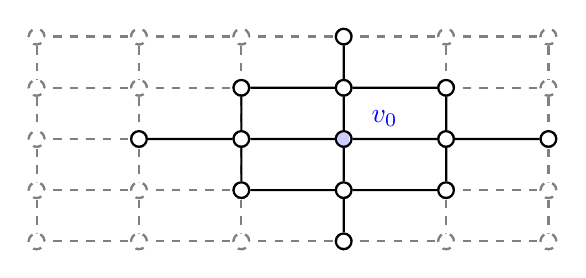
\begin{tikzpicture}[thick, scale = 1.3]
      \tikzstyle{every node} = [inner sep = 2pt];
      \foreach \x in {0,...,5}{
        \foreach \y in {0,...,4}{
          \node [draw, circle, dashed, black!50] at (\x, \y/2) {};
        }
      }
      \foreach \x in {0,...,4}{
        \foreach \y in {0,...,4}{
          \path[-]
          (\x,\y/2) edge[dashed, black!50] (\x+1,\y/2);
        }
      }
      \foreach \x in {0,...,5}{
        \foreach \y in {0,...,3}{
          \path[-]
          (\x,\y/2) edge[dashed, black!50] (\x,\y/2 + 1/2);
        }
      }
      \foreach \x in {0,...,5}{
        \foreach \y in {0,...,4}{
          \node [draw = black!50, dashed, circle,fill=white] at (\x, \y/2) {};
        }
      }
      \node[fill=blue!20!white] at (3,1){};
      \node at (3.4,1.2){\textcolor{blue}{$v_0$}};
      \node(bb) [draw, circle] at (3, 0) {};
      \node(s) [draw, circle] at (3, 1) {};
      \node(b) [draw, circle] at (3, 0.5) {};
      \node(u) [draw, circle] at (3, 1.5) {};
      \node(uu) [draw, circle] at (3, 2) {};
      \node(l) [draw, circle] at (2, 1) {};
      \node(lb) [draw, circle] at (2, 0.5) {};
      \node(lu) [draw, circle] at (2, 1.5) {};
      \node(r) [draw, circle] at (4, 1) {};
      \node(rb) [draw, circle] at (4, 0.5) {};
      \node(ru) [draw, circle] at (4, 1.5) {};
      \node(ll) [draw, circle] at (1, 1) {};
      \node(rr) [draw, circle] at (5, 1) {};
      \path[]
      (s) edge (u)
      edge (l)
      edge (b)
      edge (r)
      (l) edge (ll)
      edge (lu)
      edge (lb)
      (r) edge (rr)
      edge (ru)
      edge (rb)
      (u) edge (uu)
      edge (lu)
      edge (ru)
      (b) edge (bb)
      edge (lb)
      edge (rb);
    \end{tikzpicture}
  \end{center}
  \caption{Grid graph (in dashed grey) and the subgraph induced by $N_2(v_0)$ (in black).}
  \label{fig:gridgraph}
\end{figure}
\begin{figure}[h!t]
  \begin{center}
    \begin{tikzpicture}[thick,scale=1.5]
      \begin{scope}[scale=1.0]
        \tikzstyle{every node} = [inner sep=2pt]
        \node[fill=black, circle] at (3,1){};
        \node(bb) [draw, circle] at (3, 0) {};
        \node(s) [draw, circle] at (3, 1) {};
        \node(b) [draw, circle] at (3, 0.5) {};
        \node(u) [draw, circle] at (3, 1.5) {};
        \node(uu) [draw, circle] at (3, 2) {};
        \node(l) [draw, circle] at (2.5, 1) {};
        \node(lb) [draw, circle] at (2.5, 0.5) {};
        \node(lu) [draw, circle] at (2.5, 1.5) {};
        \node(r) [draw, circle] at (3.5, 1) {};
        \node(rb) [draw, circle] at (3.5, 0.5) {};
        \node(ru) [draw, circle] at (3.5, 1.5) {};
        \node(ll) [draw, circle] at (2, 1) {};
        \node(rr) [draw, circle] at (4, 1) {};
        \path[black!50, dashed]
        (s) edge (u)
        edge (l)
        edge (b)
        edge (r)
        (l) edge (ll)
        edge (lu)
        edge (lb)
        (r) edge (rr)
        edge (ru)
        edge (rb)
        (u) edge (uu)
        edge (lu)
        edge (ru)
        (b) edge (bb)
        edge (lb)
        edge (rb);
        \path[->,>=stealth']
        (s) edge (r)
        (r) edge (rr)
        (u) edge (ru)
        (b) edge (rb)
        (l) edge (s)
        ;
      \end{scope}
      \begin{scope}[xshift=2cm,scale=1.0]
        \tikzstyle{every node} = [inner sep=2pt]
      \node[fill=black, circle] at (3,1){};
      \node(bb) [draw, circle] at (3, 0) {};
      \node(s) [draw, circle] at (3, 1) {};
      \node(b) [draw, circle] at (3, 0.5) {};
      \node(u) [draw, circle] at (3, 1.5) {};
      \node(uu) [draw, circle] at (3, 2) {};
      \node(l) [draw, circle] at (2.5, 1) {};
      \node(lb) [draw, circle] at (2.5, 0.5) {};
      \node(lu) [draw, circle] at (2.5, 1.5) {};
      \node(r) [draw, circle] at (3.5, 1) {};
      \node(rb) [draw, circle] at (3.5, 0.5) {};
      \node(ru) [draw, circle] at (3.5, 1.5) {};
      \node(ll) [draw, circle] at (2, 1) {};
      \node(rr) [draw, circle] at (4, 1) {};
      \path[black!50, dashed]
      (s) edge (u)
      edge (l)
      edge (b)
      edge (r)
      (l) edge (ll)
      edge (lu)
      edge (lb)
      (r) edge (rr)
      edge (ru)
      edge (rb)
      (u) edge (uu)
      edge (lu)
      edge (ru)
      (b) edge (bb)
      edge (lb)
      edge (rb);
      \path[->,>=stealth']
      (s) edge (l)
      (r) edge (s)
      (u) edge (lu)
      (b) edge (lb)
      (l) edge (ll)
      ;
      \end{scope}
      \begin{scope}[xshift=4cm, scale=1.0]
        \tikzstyle{every node} = [inner sep=2pt]
        \node[fill=black, circle] at (3,1){};
        \node(bb) [draw, circle] at (3, 0) {};
        \node(s) [draw, circle] at (3, 1) {};
        \node(b) [draw, circle] at (3, 0.5) {};
        \node(u) [draw, circle] at (3, 1.5) {};
        \node(uu) [draw, circle] at (3, 2) {};
        \node(l) [draw, circle] at (2.5, 1) {};
        \node(lb) [draw, circle] at (2.5, 0.5) {};
        \node(lu) [draw, circle] at (2.5, 1.5) {};
        \node(r) [draw, circle] at (3.5, 1) {};
        \node(rb) [draw, circle] at (3.5, 0.5) {};
        \node(ru) [draw, circle] at (3.5, 1.5) {};
        \node(ll) [draw, circle] at (2, 1) {};
        \node(rr) [draw, circle] at (4, 1) {};
        \path[black!50, dashed]
        (s) edge (u)
        edge (l)
        edge (b)
        edge (r)
        (l) edge (ll)
        edge (lu)
        edge (lb)
        (r) edge (rr)
        edge (ru)
        edge (rb)
        (u) edge (uu)
        edge (lu)
        edge (ru)
        (b) edge (bb)
        edge (lb)
        edge (rb);
        \path[->,>=stealth']
        (s) edge (u)
        (r) edge (ru)
        (u) edge (uu)
        (b) edge (s)
        (l) edge (lu)
        ;
      \end{scope}
      \begin{scope}[xshift=6cm, scale=1.0]
        \tikzstyle{every node} = [inner sep=2pt]
        \node[fill=black, circle] at (3,1){};
        \node(bb) [draw, circle] at (3, 0) {};
        \node(s) [draw, circle] at (3, 1) {};
        \node(b) [draw, circle] at (3, 0.5) {};
        \node(u) [draw, circle] at (3, 1.5) {};
        \node(uu) [draw, circle] at (3, 2) {};
        \node(l) [draw, circle] at (2.5, 1) {};
        \node(lb) [draw, circle] at (2.5, 0.5) {};
        \node(lu) [draw, circle] at (2.5, 1.5) {};
        \node(r) [draw, circle] at (3.5, 1) {};
        \node(rb) [draw, circle] at (3.5, 0.5) {};
        \node(ru) [draw, circle] at (3.5, 1.5) {};
        \node(ll) [draw, circle] at (2, 1) {};
        \node(rr) [draw, circle] at (4, 1) {};
        \path[black!50, dashed]
        (s) edge (u)
        edge (l)
        edge (b)
        edge (r)
        (l) edge (ll)
        edge (lu)
        edge (lb)
        (r) edge (rr)
        edge (ru)
        edge (rb)
        (u) edge (uu)
        edge (lu)
        edge (ru)
        (b) edge (bb)
        edge (lb)
        edge (rb);
        \path[->,>=stealth']
        (s) edge (b)
        (r) edge (rb)
        (u) edge (s)
        (b) edge (bb)
        (l) edge (lb)
        ;
      \end{scope}
    \end{tikzpicture}
  \end{center}
  \caption{Translations (black arrows) in the induced subgraph (dashed grey) around $v_0$ (filled in black) that contains $v_0$ and only some of its neighbors.}
  \label{fig:inducedtranslations}
\end{figure}


\paragraph{Second step: move a small localized kernel}

Given an arbitrary\footnote{In practice we run several experiments while changing the initial vertex and keep the best obtained result.} vertex $v_0 \in V$, we place an indexing kernel on $N_1(v_0)$ i.e. $N_1(v_0) = \{v_0, v_1, ..., v_{\kappa-1}\}$. Then we move it using every local translations of center $v_0$, repeating this process for each center that is reached for the first time. We stop when the kernel has been moved everywhere in the graph. In case of multiple paths leading to the same destination, we keep the indexing that minimizes the sum of loss of the series of local translations. We henceforth obtain an indexing of at most $\kappa$ objects of $N_1(v)$ for every $v \in V$.

This process is depicted in \figref{fig:movekernel}. Since it requires moving the kernel everywhere, its complexity is $\mathcal{O}(n d^2)$.

\begin{figure}[h!p]
  \begin{center}
    \begin{tikzpicture}[thick]
      \begin{scope}[scale=0.8]
        \node at (-1,2) {a)};
        \foreach \x in {0,...,5}{
          \foreach \y in {0,...,4}{
            \node [draw, circle, dashed, black!50] at (\x, \y) {};
          }
        }
        \foreach \x in {0,...,4}{
          \foreach \y in {0,...,4}{
            \path[-]
            (\x,\y) edge[dashed, black!50] (\x+1,\y);
          }
        }
        \foreach \x in {0,...,5}{
          \foreach \y in {0,...,3}{
            \path[-]
            (\x,\y) edge[dashed, black!50] (\x,\y + 1);
          }
        }
        \foreach \x in {0,...,5}{
          \foreach \y in {0,...,4}{
            \node(\x\y) [draw = black!50, dashed, circle,fill=white] at (\x, \y) {};
          }
        }
        \node at (3,2){$v_0$};
        \node at (2,2){$v_1$};
        \node at (1,2){$v_2$};
        \node at (1,3){$v_3$};

        \node[draw = black, circle] at (3,2){};
        \node[draw = red, circle] at (2,2){};
        \node[draw = green!50!black, circle] at (4,2){};
        \node[draw = blue, circle] at (3,3){};
        \node[draw = purple, circle] at (3,1){};
      \end{scope}
      \begin{scope}[xshift=5cm, scale=0.8]
        \node at (-1,2) {b)};
        \foreach \x in {0,...,5}{
          \foreach \y in {0,...,4}{
            \node [draw, circle, dashed, black!50] at (\x, \y) {};
          }
        }
        \foreach \x in {0,...,4}{
          \foreach \y in {0,...,4}{
            \path[-]
            (\x,\y) edge[dashed, black!50] (\x+1,\y);
          }
        }
        \foreach \x in {0,...,5}{
          \foreach \y in {0,...,3}{
            \path[-]
            (\x,\y) edge[dashed, black!50] (\x,\y + 1);
          }
        }
        \foreach \x in {0,...,5}{
          \foreach \y in {0,...,4}{
            \node(\x\y) [draw = black!50, dashed, circle,fill=white] at (\x, \y) {};
          }
        }
        \node at (3,2){$v_0$};
        \node at (2,2){$v_1$};
        \node at (1,2){$v_2$};
        \node at (1,3){$v_3$};
        \draw
        (0.5,2) -- (3,4.5) -- (5.5,2) -- (3,-0.5) -- (0.5,2);
        \path[->,>=stealth']
        (31) edge (21)
        (32) edge (22)
        (33) edge (23)
        (42) edge (32)
        (22) edge (12);
        \node[draw = black, circle] at (2,2){};
        \node[draw = red, circle] at (1,2){};
        \node[draw = green!50!black, circle] at (3,2){};
        \node[draw = blue, circle] at (2,3){};
        \node[draw = purple, circle] at (2,1){};
      \end{scope}
      \begin{scope}[scale=0.8, yshift=-6cm]
        \node at (-1,2) {c)};
        \foreach \x in {0,...,5}{
          \foreach \y in {0,...,4}{
            \node [draw, circle, dashed, black!50] at (\x, \y) {};
          }
        }
        \foreach \x in {0,...,4}{
          \foreach \y in {0,...,4}{
            \path[-]
            (\x,\y) edge[dashed, black!50] (\x+1,\y);
          }
        }
        \foreach \x in {0,...,5}{
          \foreach \y in {0,...,3}{
            \path[-]
            (\x,\y) edge[dashed, black!50] (\x,\y + 1);
          }
        }
        \foreach \x in {0,...,5}{
          \foreach \y in {0,...,4}{
            \node(\x\y) [draw = black!50, dashed, circle,fill=white] at (\x, \y) {};
          }
        }
        \node at (3,2){$v_0$};
        \node at (2,2){$v_1$};
        \node at (1,2){$v_2$};
        \node at (1,3){$v_3$};
        \draw
        (-0.5,2) -- (2,4.5) -- (4.5,2) -- (2,-0.5) -- (-0.5,2);
        \path[->,>=stealth']
        (21) edge (11)
        (22) edge (12)
        (23) edge (13)
        (32) edge (22)
        (12) edge (02);
        \node[draw = black, circle] at (1,2){};
        \node[draw = red, circle] at (0,2){};
        \node[draw = green!50!black, circle] at (2,2){};
        \node[draw = blue, circle] at (1,3){};
        \node[draw = purple, circle] at (1,1){};
      \end{scope}
      
      \begin{scope}[xshift=5cm, scale=0.8,yshift=-6cm]
        \node at (-1,2) {d)};
        \foreach \x in {0,...,5}{
          \foreach \y in {0,...,4}{
            \node [draw, circle, dashed, black!50] at (\x, \y) {};
          }
        }
        \foreach \x in {0,...,4}{
          \foreach \y in {0,...,4}{
            \path[-]
            (\x,\y) edge[dashed, black!50] (\x+1,\y);
          }
        }
        \foreach \x in {0,...,5}{
          \foreach \y in {0,...,3}{
            \path[-]
            (\x,\y) edge[dashed, black!50] (\x,\y + 1);
          }
        }
        \foreach \x in {0,...,5}{
          \foreach \y in {0,...,4}{
            \node(\x\y) [draw = black!50, dashed, circle,fill=white] at (\x, \y) {};
          }
        }
        \node at (3,2){$v_0$};
        \node at (2,2){$v_1$};
        \node at (1,2){$v_2$};
        \node at (1,3){$v_3$};
        \draw
        (-1.5,2) -- (1,4.5) -- (3.5,2) -- (1,-0.5) -- (-1.5,2);
        \path[->,>=stealth']
        (11) edge (12)
        (12) edge (13)
        (13) edge (14)
        (22) edge (23)
        (02) edge (03);
        \node[draw = black, circle] at (1,3){};
        \node[draw = red, circle] at (0,3){};
        \node[draw = green!50!black, circle] at (2,3){};
        \node[draw = blue, circle] at (1,4){};
        \node[draw = purple, circle] at (1,2){};
      \end{scope}
    \end{tikzpicture}
  \end{center}
  \caption{Illustration of the translation of a small indexing kernel using translations in each induced subgraph. Kernel is initialized around $v_0$ (a), then moved left around $v_1$ (b) using the induced subgraph around $v_0$, then moved left again around $v_2$ (c) using the induced subgraph around $v_1$ then moved up around $v_3$ (d) using the induced subgraph around $v_2$. At the end of the process, the kernel has been localized around each vertex in the graph.}
  \label{fig:movekernel}
\end{figure}


\paragraph{Final step: identifying proxy-translations}

Finally, by looking at the indexings obtained in the previous step, we obtain a family of proxy-translations defined globally on $G$. More precisely, each index defines its own proxy-translation. Note that they are not translations because only the local properties have been propagated through the second step, so there can exist aligned candidates with smaller losses. Because of the constraint to keep the paths with the minimum sum of losses, they are good proxies to translations on $G$.

An illustration on a grid graph is given in \figref{fig:translations}. The complexity is $\mathcal{O}(nd)$. Overall, all three steps are linear in $n$.

\begin{figure}[h!p]
  \begin{center}
    \begin{tikzpicture}[thick,scale=0.8]
      \tikzstyle{every node} = [inner sep = 2pt];
      \begin{scope}
        \foreach \x in {0,...,5}{
          \foreach \y in {0,...,4}{
            \node(\x\y) [draw, circle, black] at (\x, \y/2) {};
          }
        }
        \foreach \x in {0,...,4}{
          \foreach \y in {0,...,4}{
            \pgfmathtruncatemacro{\nouveaux}{\x+1}
            \path[->,>=stealth']            
            (\x\y) edge[bend left, green!50!black] (\nouveaux\y);
          }
        }
        \foreach \x in {0,...,5}{
          \foreach \y in {0,...,3}{
            \pgfmathtruncatemacro{\nouveauy}{\y+1}
            \path[->,>=stealth']
            (\x\y) edge[bend left, blue] (\x\nouveauy);
          }
        }
        \foreach \x in {1,...,5}{
          \foreach \y in {0,...,4}{
            \pgfmathtruncatemacro{\nouveaux}{\x-1}
            \path[->,>=stealth']
            (\x\y) edge[bend left, red] (\nouveaux\y);
          }
        }
        \foreach \x in {0,...,5}{
          \foreach \y in {1,...,4}{
            \pgfmathtruncatemacro{\nouveauy}{\y-1}
            \path[->,>=stealth']
            (\x\y) edge[bend left, purple] (\x\nouveauy);
          }
        }
      \end{scope}
    \end{tikzpicture}
  \end{center}
  \caption{Proxy-translations in $G$ obtained after moving the small kernel around each vertex. Each color corresponds to one translation.}
  \label{fig:translations}
\end{figure}

\subsection{Subsampling}

Downscaling is a tricky part of the process because it supposes one can somehow regularly sample vectors. As a matter of fact, a non-regular sampling is likely to produce a highly irregular downscaled graph, on which looking for translations irremediably leads to poor accuracy, as we noticed in our experiments.% Instead, here we propose to use translations on $G$ to define the extended downscaling layers. They basically are obtained by masking vertices in the initial graph.

We rather define the translations of the strided graph using the previously found proxy-translations on $G$.

\paragraph{First step: extended convolution with stride $r$}
%\subsubsection{First step: convolution with stride $r$}
%Here we define an extended convolution layer with stride $r$.

Given an arbitrary initial vertex $v_0 \in V$, the set of kept vertices $V_{\downarrow r}$ is defined inductively as follows:
\begin{itemize}[noitemsep,nolistsep]
\item $V_{\downarrow r}^0 = \{v_0\}$,
\item $\forall t \in \mathbb{N}, V_{\downarrow r}^{t+1} = V_{\downarrow r}^t \cup \{v \in V, \forall v' \in V_{\downarrow }^t, v \not\in N_{r-1}(v') \land \exists v' \in V_{\downarrow r}^t, v \in N_{r}(v') \}$.
\end{itemize}
This sequence is non-decreasing and bounded by $V$, so it eventually becomes stationary and we obtain $V_{\downarrow r} = \lim_t{V_{\downarrow r}^t}$. $V_{\downarrow r}$ is the set of output neurons of the extended convolution layer with stride~$r$. \figref{fig:downscaling} illustrate the first downscaling $V_{\downarrow 2}$ on a grid graph. %% $V_{\downarrow 2}$ is used to define the stride in extended convolution layers.

\paragraph{Second step: convolutions for the strided graph}

Using the proxy-translations on $G$, we move a localized $r$-hop indexing kernel over $G$. At each location, we associate the vertices of $V_{\downarrow r}$ with indices of the kernel, thus obtaining what we define as induced $_{\downarrow r}$-translations on the set $V_{\downarrow r}$. In other words, when the kernel is centered on $v_0$, if $v_1 \in V_{\downarrow r}$ is associated with the index $p_0$, we obtain $\phi_{p_0}^{\downarrow r}(v_0) = v_1$. Subsequent convolutions at lower scales are defined using these induced $_{\downarrow r}$-translations.
%The downstream convolution's weight-sharing schemes are then obtained by moving a kernel covering the full graph to each vertex in $V_{\downarrow r}$, similarly to Subsection C.

%% Note that every downscaling layers of the extended architecture are defined from the translation found on the graph at the input level of the network. A typical extended CNN architecture would contain ${2^r}$ downscaled layers.

\begin{figure}[h!]
  \begin{center}
    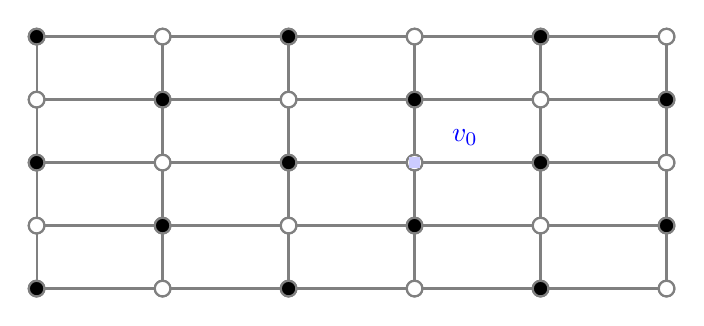
\begin{tikzpicture}[thick, scale=1.6]
      \tikzstyle{every node} = [inner sep = 2pt];
      \foreach \x in {0,...,5}{
        \foreach \y in {0,...,4}{
          \node [draw, circle, black!50] at (\x, \y/2) {};
        }
      }
      \foreach \x in {0,...,4}{
        \foreach \y in {0,...,4}{
          \path[-]
          (\x,\y/2) edge[black!50] (\x+1,\y/2);
        }
      }
      \foreach \x in {0,...,5}{
        \foreach \y in {0,...,3}{
          \path[-]
          (\x,\y/2) edge[black!50] (\x,\y/2 + 1/2);
        }
      }
      \foreach \x in {0,...,5}{
        \foreach \y in {0,...,4}{
          \pgfmathtruncatemacro{\sum}{\x+\y}
          \ifodd\sum
          \node(\x\y) [draw = black!50, circle,fill=white] at (\x, \y/2) {};
          \else
          \node(\x\y) [draw = black!50, circle,fill=black] at (\x, \y/2) {};
          \fi
        }
      }
      \node at (3.4,1.2){\textcolor{blue}{$v_0$}};
      \node[fill=blue!20!white] at (3,1){};
    \end{tikzpicture}
  \end{center}
  
  \caption{Downscaling of the grid graph. Disregarded vertices are filled in.}
  \label{fig:downscaling}
\end{figure}

\subsection{Data augmentation}

Once proxy-translations are obtained on $G$, we use them to move training signals, artificially creating new ones. Note that this type of data-augmentation is weaker than for images since no flipping, scaling or rotations are used.

\subsection{Experiments}

\paragraph{Matching CNNs on supervised image classification}
On CIFAR-$10$ (see \secref{sec:datasets}), our models are based on a variant of a deep residual network, namely PreActResNet18 \citep{he2016identity}. We tested different combinations of graph support and data augmentation. For the graph support, we use either a regular 2D grid or either an inferred graph obtained by keeping the four neighbors that covary the most. In the second case, which correspond to scrambled CIFAR-$10$ (see \secref{sec:datasets}), no structure prior have been fed to the process, so the results can be compared with those of \cite{lin2015}. We also report results obtained with ChebNet~\citep{defferrard2016convolutional}, where only convolutional layers have been replaced for comparison. \tabref{tab:cifar-table} summarizes our results. In particular, it is interesting to note that results obtained without any structure prior (91.07\%) are only 2.7\% away from the baseline using classical CNNs on images (93.80\%). This gap is even smaller (less than 1\%) when using the grid prior. Also, on scrambled CIFAR-$10$ (case without prior) our method significantly outperforms the others.%% In the top left corner of the table we fully exploit the fact that the dataset is composed of 2D structured data, and in the bottom right corner this information is not used at all. Even with that disadvantage, the results differ of only 2.7\%, which shows the strenght of the method when compared to others.

\begin{table}[h!]
\begin{center}
\caption{CIFAR-$10$ and scrambled CIFAR-$10$ comparison table.}
\vspace{-0.4cm}
\label{tab:cifar-table}
\resizebox{\columnwidth}{!}{%
\begin{tabular}{|l|c|c|c|c|c|}
\hline
\multirow{2}{*}{Support} & \multirow{2}{*}{MLP} %\multirow{2}{*}{\begin{tabular}[c]{@{}c@{}}MLP \\\citeauthor{lin2015}\end{tabular}}
& \multirow{2}{*}{CNN} & \multicolumn{2}{c|}{Grid Graph}       & Covariance Graph         \\ \cline{4-6} 
                         &                                                                                &                      & ChebNet$^c$ & Proposed & Proposed              \\ \hline
Full Data Augmentation   & 78.62\%$^{a,b}$                                                                     & \textbf{93.80\%}     & 85.13\%                            & 93.94\%  & 92.57\%                                         \\ \hline
Data Augmentation - Flip & ------                                                                         & 92.73\%              & 84.41\%                            & 92.94\%  & 91.29\%                                         \\ \hline
Graph Data Augmentation  & ------                                                                         & 92.10\%$^d$          & ------                             & 92.81\%  & \textbf{91.07\%}$^a$                             \\ \hline
None                     & 69.62\%                                                                        & 87.78\%              & ------                             & 88.83\%  & 85.88\%$^a$                                      \\\hline
\end{tabular}

}
%\vspace{-0.2cm}
\end{center}
\begin{flushleft}
\footnotesize{
$^a$ No prior about the structure\\
$^b$ \cite{lin2015}\\
$^c$ \cite{defferrard2016convolutional}\\
$^d$ Data augmentation done with covariance graph 
}
\end{flushleft}
\end{table}

\paragraph{Experiments on a fMRI dataset}
We used a shallow network on the PINES dataset (see \secref{sec:datasets}). The results reported on \tabref{tab:iaps-table} show that our method was able to improve over CNNs, MLPs and other graph-based extended convolutional neural networks.

\begin{table}[h!]
\centering
\caption{PINES fMRI comparison table.}
\label{tab:iaps-table}
\begin{tabular}{|l||c|c||c|c|}
\hline
\multicolumn{1}{|l||}{Support} & \multicolumn{2}{c||}{None} & \multicolumn{2}{c|}{Neighborhood Graph}     \\ \hline
Method                      & MLP & CNN (1x1 kernels)                                & ChebNet$^c$ & Proposed                   \\ \hline
Accuracy                    & 82.62\% & 84.30\%                            & 82.80\%                            & \textbf{85.08\%} \\ \hline
\end{tabular}
%\vspace{-.4cm}
\end{table}

